\documentclass[aspectratio=169]{beamer}
\usetheme{metropolis}
\usecolortheme{default}

\usepackage{color}
\usepackage{graphicx}
\usepackage{amssymb}
\usepackage{amsmath}
\usepackage{wasysym}
\usepackage{tabularx, booktabs}
\usepackage[lined]{algorithm2e}

% For text bubble
\usepackage{tikz}
\usetikzlibrary{shapes,fit,backgrounds}
\newcounter{mybox}
\newcommand\tikzmark[1]{%
  \tikz[remember picture,overlay] \node[inner xsep=0pt] (#1) {};
}
\newcommand<>\ColorBox[2][]{%
\stepcounter{mybox}%
\node[rectangle callout,rounded corners=5pt,draw=cyan,fill=cyan!20,align=left,#1] (box\themybox) {#2};
}

%\usepackage{bibentry}
%\nobibliography*

% metropolis beamer theme can be found in GitHub:
% https://github.com/matze/mtheme

\title{EEL6935 Course Project\\ Final Report}
\author[Bryant, Feng]{Caleb~Bryant\inst{1}\and Jixin~Feng\inst{2}}
\institute{
Department of \\
  \inst{1}
  Computer \& Information Science \& Engineering \\
  \inst{2}
  Electrical \& Computer Engineering\\
  University of Florida, Gainesville, FL}
\date{EEL6935 T21}

\begin{document}
\frame{\titlepage}

%\begin{frame}
%\frametitle{Background}
%    \begin{columns}
%    \begin{column}{0.5\textwidth}
%    \begin{itemize}
%        \item Tremendous volume of unstructured text generated everyday
%        \item 40ZB ($40\times 10^{21}$bytes) by year 2020, 50-fold from 2010\footnotemark
%        \item generated from news media, social networks, medical records, 
%            business transactions\ldots
%        \item effective processing method is needed
%    \end{itemize}
%    \end{column}
%    \begin{column}{0.5\textwidth}
%    \center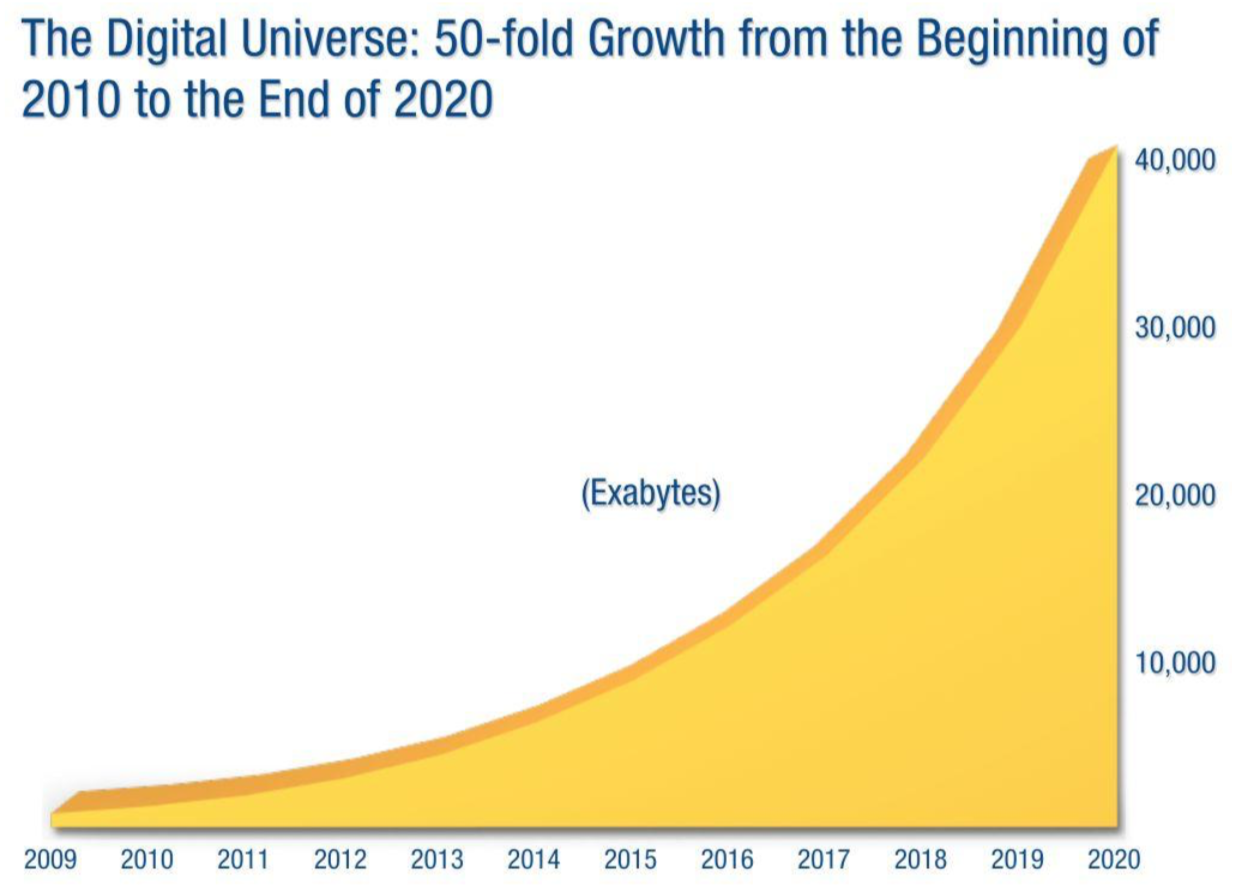
\includegraphics[width=\textwidth]{figure/data_growth_2020}
%    \end{column}
%    \end{columns}
%    \footnotetext[1]{Gantz, J., \& Reinsel, D. (2012). The digital universe in 2020: Big data, bigger digital shadows, and biggest growth in the far east. IDC iView: IDC Analyze the future, 2007(2012), 1-16.}
%\end{frame}

\begin{frame}
\frametitle{Sentiment Analysis}
    \begin{columns}
    \begin{column}{0.6\textwidth}
    Goal: assign sentiment labels to a sentence.
    $f:\mathcal{D}\rightarrow\mathcal{L}$
    \begin{itemize}
        \item $\mathcal{D}=\{d_0, d_1,\ldots, d_{n-1}\}$ is the set of sentence
        \item $\mathcal{L}=\{l_0, l_1,\ldots, l_{k-1}\}$ is the set of labels.
    \end{itemize}
    Movie review is ideal for sentiment analysis
    \begin{itemize}
        \item Most dataset of movie review are already associated with scores
        \item The scores in dataset are reliable
    \end{itemize}
    \end{column}
    \begin{column}{0.4\textwidth}
    \center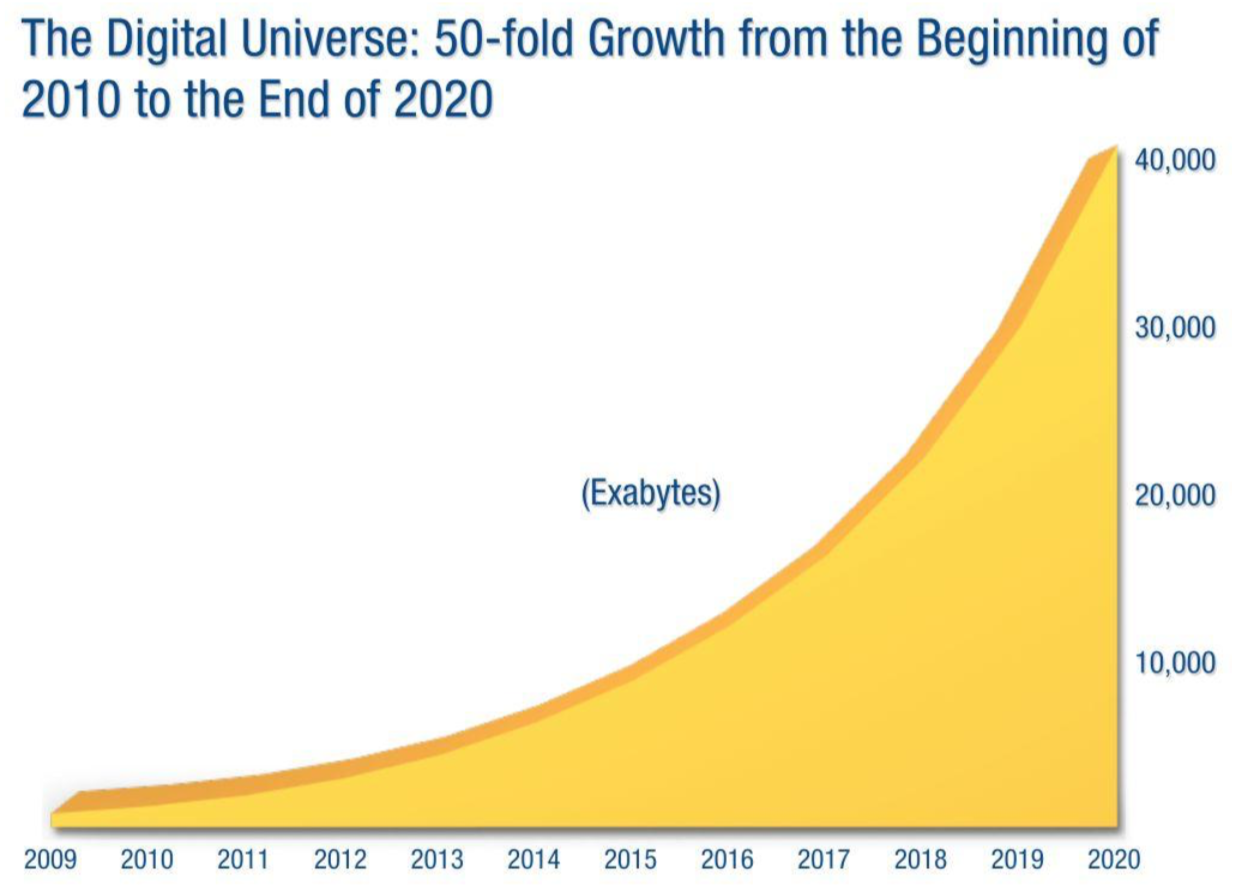
\includegraphics[width=\textwidth]{figure/data_growth_2020}
    \end{column}
    \end{columns}
    \footnotetext[1]{Gantz, J., \& Reinsel, D. (2012). The digital universe in 2020: Big data, bigger digital shadows, and biggest growth in the far east. IDC iView: IDC Analyze the future, 2007(2012), 1-16.}
\end{frame}

%\begin{frame}
%\frametitle{Text Pre-processing}
%    \begin{columns}
%    \begin{column}{0.4\textwidth}
%    \center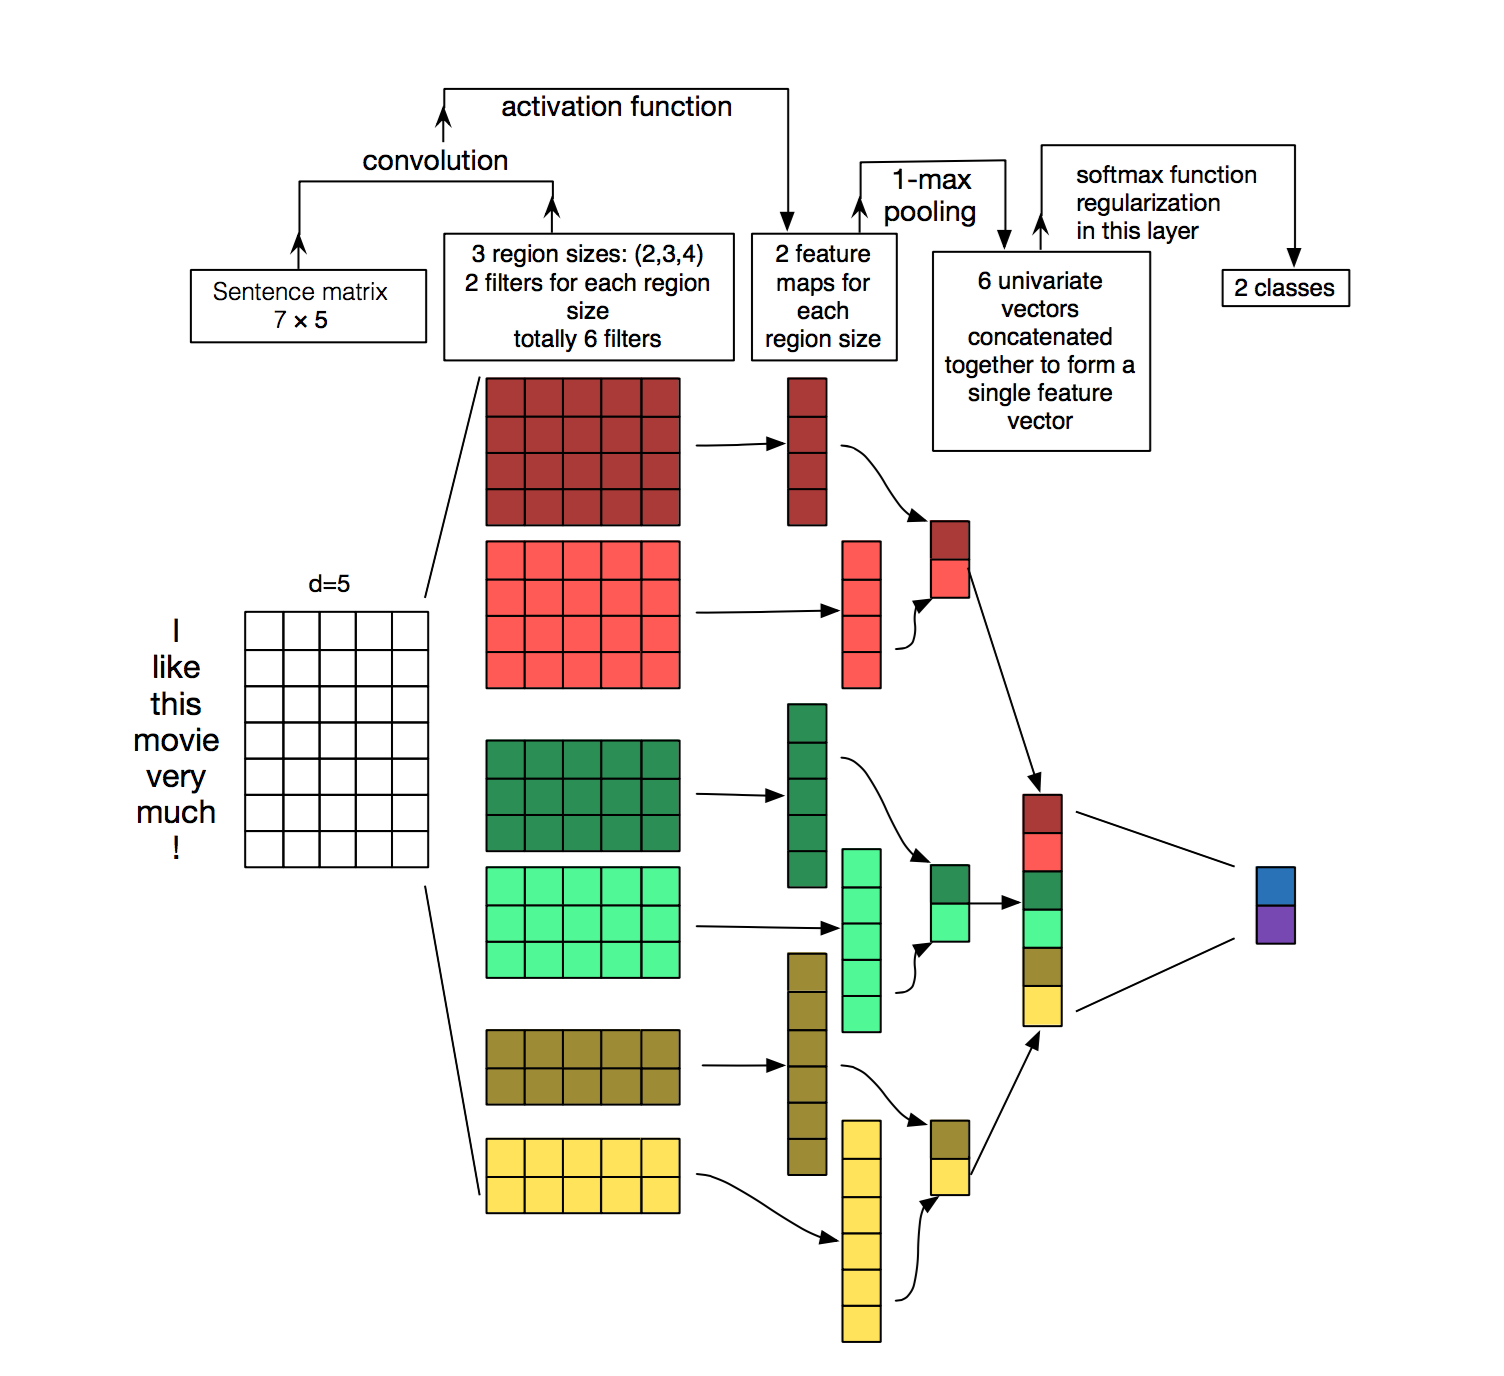
\includegraphics[width=\textwidth]{figure/sc_cnn}
%    \end{column}
%    \begin{column}{0.6\textwidth}
%    \begin{itemize}
%        \item Tokenization
%        \begin{itemize}
%            \item Remove the unnecessary parts of the text
%            \item Break the text into smaller building blocks like words and phrases
%        \end{itemize}
%        \item Filtering
%        \begin{itemize}
%            \item emove the part of the text that convey close to zero information
%        \end{itemize}
%        \item Lemmatization
%        \begin{itemize}
%            \item Groups the words within same role of the text together
%        \end{itemize}
%        \item Stemming
%        \begin{itemize}
%            \item Find a root of text first and create the tree
%             structure to represent their relationship
%        \end{itemize}
%    \end{itemize}
%    \end{column}
%    \end{columns}
%    \footnotetext{figure credit: http://www.wildml.com/2015/11/understanding-convolutional-neural-networks-for-nlp/}
%\end{frame}

\begin{frame}
\frametitle{Text Encoding}
    \begin{itemize}
        \item Define the collection of text documents to be 
            $$\mathcal{D}=\{d_1, d_2,\ldots,d_D\}$$
        \item Define vocabulary to be
            $$\mathcal{V}=\{v_0, v_1,\ldots, v_{m-1}\}$$
        \item The notation of frequency of a word $v\in\mathcal{V}$ occurred 
            in document $d\in\mathcal{D}$ is $f_d(v)$, hence a document can be represented as
            a vector $$\bar{d}=\{f_d(v_1),f_d(v_2),\ldots\}$$
        \item Define total number of documents
            $d\in\mathcal{D}$ containing the word $w$ is represented as $$f_\mathcal{D}(v)$$
    \end{itemize}
\end{frame}

%\begin{frame}
%\frametitle{Text Encoding}
%    Documents and words can also be assigned with other metrics
%    \begin{itemize}
%        \item Boolean weight
%            $$\omega_{ij} = 
%            \begin{cases} 
%                1 & v_i \in d_j\\
%                0 & v_i \notin d_j
%            \end{cases}$$
%        \item Term Frequency-inverse Document Frequency (TF-IDF)
%            $$q(v)=f_d(v)\log\frac{\left|\mathcal{D}\right|}{f_\mathcal{D}(v)}$$
%        \item With these weight metircs, text/document can be represented by a vector 
%            $$w(d)=(w(d,v_1),w(d,v_2),\ldots)$$
%    \end{itemize}
%\end{frame}

%\begin{frame}
%\frametitle{Evaluation}
%    \begin{columns}
%    \begin{column}{0.65\textwidth}
%    The performance can be measured by $F_1$ Score:
%    $$F_1=\frac{2}{\frac{1}{r}+\frac{1}{p}}=\frac{2pr}{p+r}$$
%    \begin{itemize}
%        \item Precision: $p=\frac{tpr}{tpr+fpr}$
%        \item Recall: $r=\frac{tpr}{tpr+fnr}$
%    \end{itemize}
%    \end{column}
%    \begin{column}{0.35\textwidth}
%        \center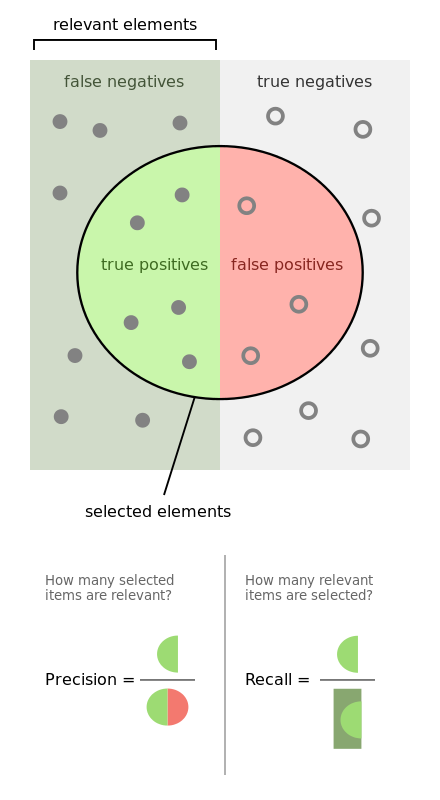
\includegraphics[width=\textwidth]{figure/precision_recall}
%    \end{column}
%    \end{columns}
%    \footnotetext{figure credit: \url{https://en.wikipedia.org/wiki/F1_score}}
%\end{frame}

%\begin{frame}
%\frametitle{Backend: Logistic Regression}
%    \begin{itemize}
%        \item $\hat{y} = \sigma(S(x^T_i W +b))$
%        \item $S(x) = \frac{1}{1+e^{-x}}$
%        \item $W$ is a $N \times C$ weight matrix
%        \item $N$ is number of words, $C$ is number of class
%        \item $\sigma (x)_{j}={\frac {e^{x_{j}}}{\sum _{i=1}^{N}e^{x_{i}}}}$
%        \item $b$ is a $C \times 1$ bias
%    \end{itemize}
%\end{frame}

\begin{frame}
\frametitle{Backend: Logistic Regression}
    \center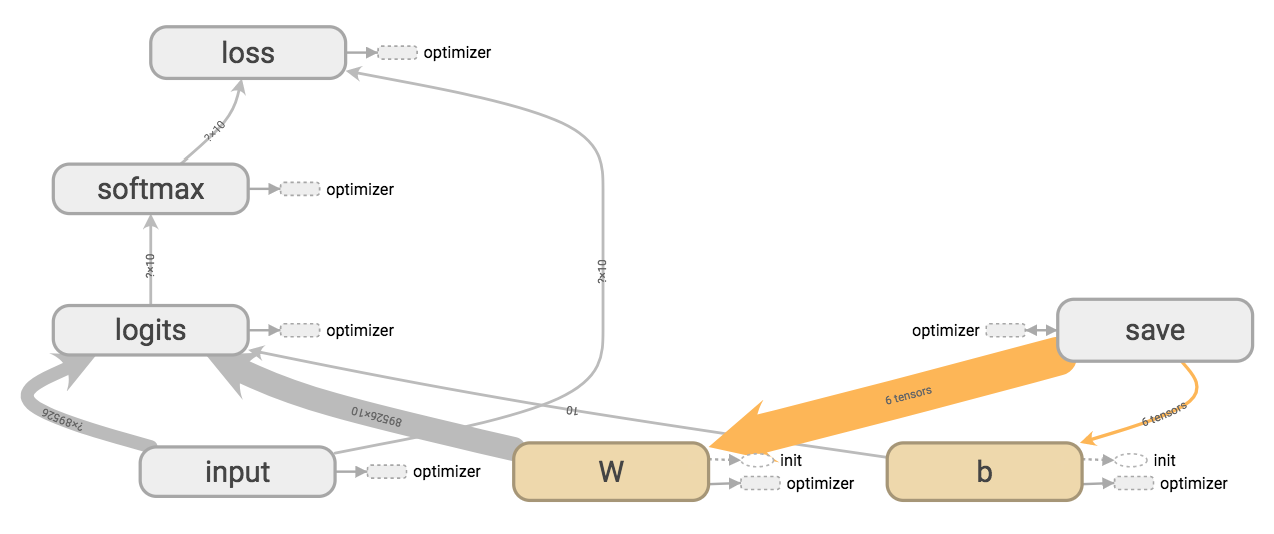
\includegraphics[width=0.7\textwidth]{figure/model_architecture}
    \begin{itemize}
        \item Multiply input vectors by $W$, add $b$
        \item Convert output into probabilities with Softmax
        \item pick $i=argmax(\hat{y}_i)$
        \item Train the model using Adam Optimizer
        \item Common baseline model and simple to implement
    \end{itemize}
\end{frame}

\begin{frame}
\frametitle{Backend: LSTM Model}
    \begin{columns}
    \begin{column}{0.4\textwidth}
    Given a word sequence $S=\{v_0,v_1,\ldots,v_{l-1}\}$ with length $l$, the states
    of LSTM are updated as:
    $$
    \begin{bmatrix} 
    i_t\\f_t\\o_t\\c_t 
    \end{bmatrix} = 
    \begin{bmatrix}
    \sigma\\\sigma\\\sigma\\\tanh
    \end{bmatrix}
    S[h_{t-1},x_t]
    $$
    \begin{itemize}
        \item $c_t=f_t\circ c_{t-1} + i_t\circ\hat{c_t}$
        \item $h_t=o_t\circ\tanh{c_t}$
    \end{itemize}

    \end{column}
    \begin{column}{0.6\textwidth}
    \center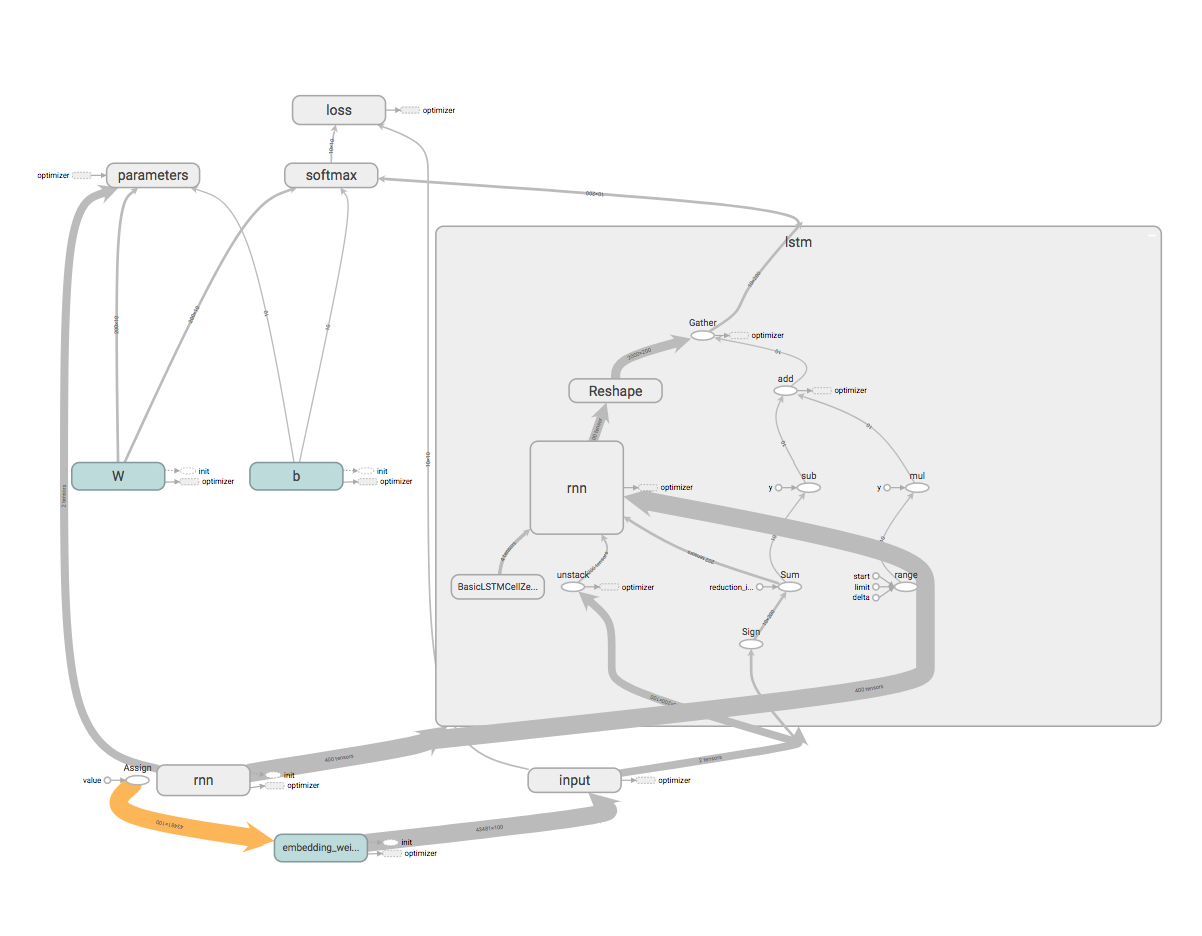
\includegraphics[width=\textwidth]{figure/lstm_architecture}
    \end{column}
    \end{columns}
\end{frame}


%\begin{frame}
%\frametitle{Backend: LSTM Model}
%    Given a word sequence $S=\{v_0,v_1,\ldots,v_{l-1}\}$ with length $l$, the states
%    of LSTM are updated as:
%    $$
%    \begin{bmatrix} 
%    i_t\\f_t\\o_t\\c_t 
%    \end{bmatrix} = 
%    \begin{bmatrix}
%    \sigma\\\sigma\\\sigma\\\tanh
%    \end{bmatrix}
%    S[h_{t-1},x_t]
%    $$
%    \begin{itemize}
%        \item $c_t=f_t\circ c_{t-1} + i_t\circ\hat{c_t}$
%        \item $h_t=o_t\circ\tanh{c_t}$
%    \end{itemize}
%\end{frame}


\begin{frame}
\frametitle{Backend: LSTM Model}
    To build our LSTM model:
    \begin{itemize}
        \item Define a dictionary 
            $$D = [w_1, w_2...w_N]$$
            to contain the set of all words representable by our LSTM network
        \item The $i$-th
            input to our LSTM is a vector
            $$
            v_i = [ \pi_{i1}, \pi_{i2}... \pi_{iL}]
            $$
            corresponding to a movie review $r_i$ of length $L$, where $\pi_{ij}$ 
            is the dictionary index of 
            the $j$-th word of $r$
        \item $D = [\text{cat}, \text{dog}, \text{meow}]$
        $$r =  [\text{dog}, \text{dog}, \text{cat}, \text{meow}]\Rightarrow v = [1, 1, 0, 2]$$
    \end{itemize}
\end{frame}

%\begin{frame}
%\frametitle{Backend: LSTM Model}
%    In order to help the LSTM learn how to interpret the words in a movie review
%    \begin{itemize}
%        \item Each sentence's words are embedded inside a weight matrix $W_e$ with
%            dimensions $N \times E$
%        \item $E$ is a hyperparameter known as the 
%            embedding dimension and often ranges between 50 and 300
%    \end{itemize}
%\end{frame}

%\begin{frame}
%\frametitle{Backend: LSTM Model}
%    After initializing the hidden state to zeros at the beginning of each batch, sequences
%    of embeddings
%    $$
%    s_i = [ e_{i1}, e_{i2}, .. e_{iL}] 
%    $$
%    are then sequentially fed into the LSTM layer of our network
%    \begin{itemize}
%        \item Each $e_{ij}$ is the embedding vector for the word $w_{ij}$ 
%        looked-up according to the input index $\pi_{ij}$
%        \item Only the final output state of the LSTM is used for prediction
%        \item It is fed into a fully-connected softmax layer
%    \end{itemize}
%\end{frame}


\begin{frame}
\frametitle{Simulation Platform Specs}
    \begin{columns}
    \begin{column}{0.6\textwidth}
    \begin{itemize}
        \item Training based on Stanford Large Movie Review Dataset
        \begin{itemize}
            \item 50,000 highly polar movie reviews
            \item 25,000 for training, 25,000 for testing
        \end{itemize}
        \item Code in Python with Tensorflow/Scikit-Learn
        \item simulations will be conducted on computers with 
        \begin{itemize}
            \item 3.1GHz Intel Core i7 CPU with 8MB cache
            \item nVidia GTX 1050 GPU with 4GB Memory
            \item 16GB RAM
            \item Ubuntu 14.04 LTS
        \end{itemize}
    \end{itemize}
    \end{column}
    \begin{column}{0.4\textwidth}
    \center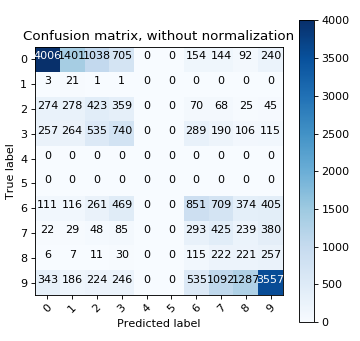
\includegraphics[width=\textwidth]{figure/conf_matrix}
    \end{column}
    \end{columns}
\end{frame}

\begin{frame}
\frametitle{Result}
    \begin{table}
        \centering
        \caption{System Performance}
        \label{my-label}
        \begin{tabularx}{\textwidth}{ X X X  X X  X }
        \toprule
        Method & Epochs & Binomial Training & Binomial Testing & Multinomial Training & Multinomial Testing \\
        \midrule
        scikit-learn LR & N/A & 0.9981 & \textbf{0.8697} & N/A & N/A \\
        tensorflow LR & 20 &  0.8670 & 0.8583 & 0.9982 & 0.3734 \\
        larger LSTM & 8 & N/A & N/A & 0.6693 & 0.3657 \\
        smaller LSTM  & 2 & N/A    & 0.8507 & 0.5622   & \textbf{0.4098} \\
        \bottomrule
        \end{tabularx}
    \end{table}
\end{frame}

%\begin{frame}
%\frametitle{Result}
%    \begin{columns}
%    \begin{column}{0.5\textwidth}
%        \center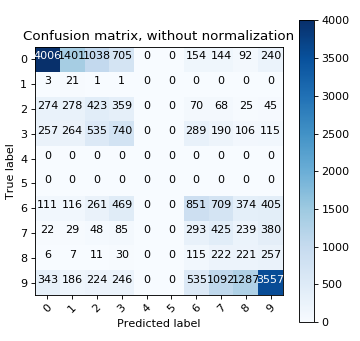
\includegraphics[width=\textwidth]{figure/conf_matrix}
%    \end{column}
%    \begin{column}{0.5\textwidth}
%        \begin{itemize}
%            \item Logistic Regression quickly converged to the global minimum
%            \item No worry about escaping local optima
%            \item LSTM is very slow to train
%            \item Need even more computational resource to achieve better accuracy
%        \end{itemize}
%    \end{column}
%    \end{columns}
%\end{frame}


\begin{frame}
\frametitle{Front End: Flask Web App}
    \begin{columns}
    \begin{column}{0.4\textwidth}
    \begin{itemize}
        \item \href{http://t21.ecegator.com}{Web App} via Flask
        \item Allow model selection
        \item Accept text input and sentiment analysis output
        \item Hosted on low spec VM
        \begin{itemize}
            \item Ubuntu 16.04 LTS
            \item Single Core CPU
            \item 2GB RAM
            \item No standalone GPU
        \end{itemize}
    \end{itemize}
%    \center
\includegraphics[width=0.4\textwidth]{figure/qr_website}
    \end{column}
    \begin{column}{0.3\textwidth}
        \center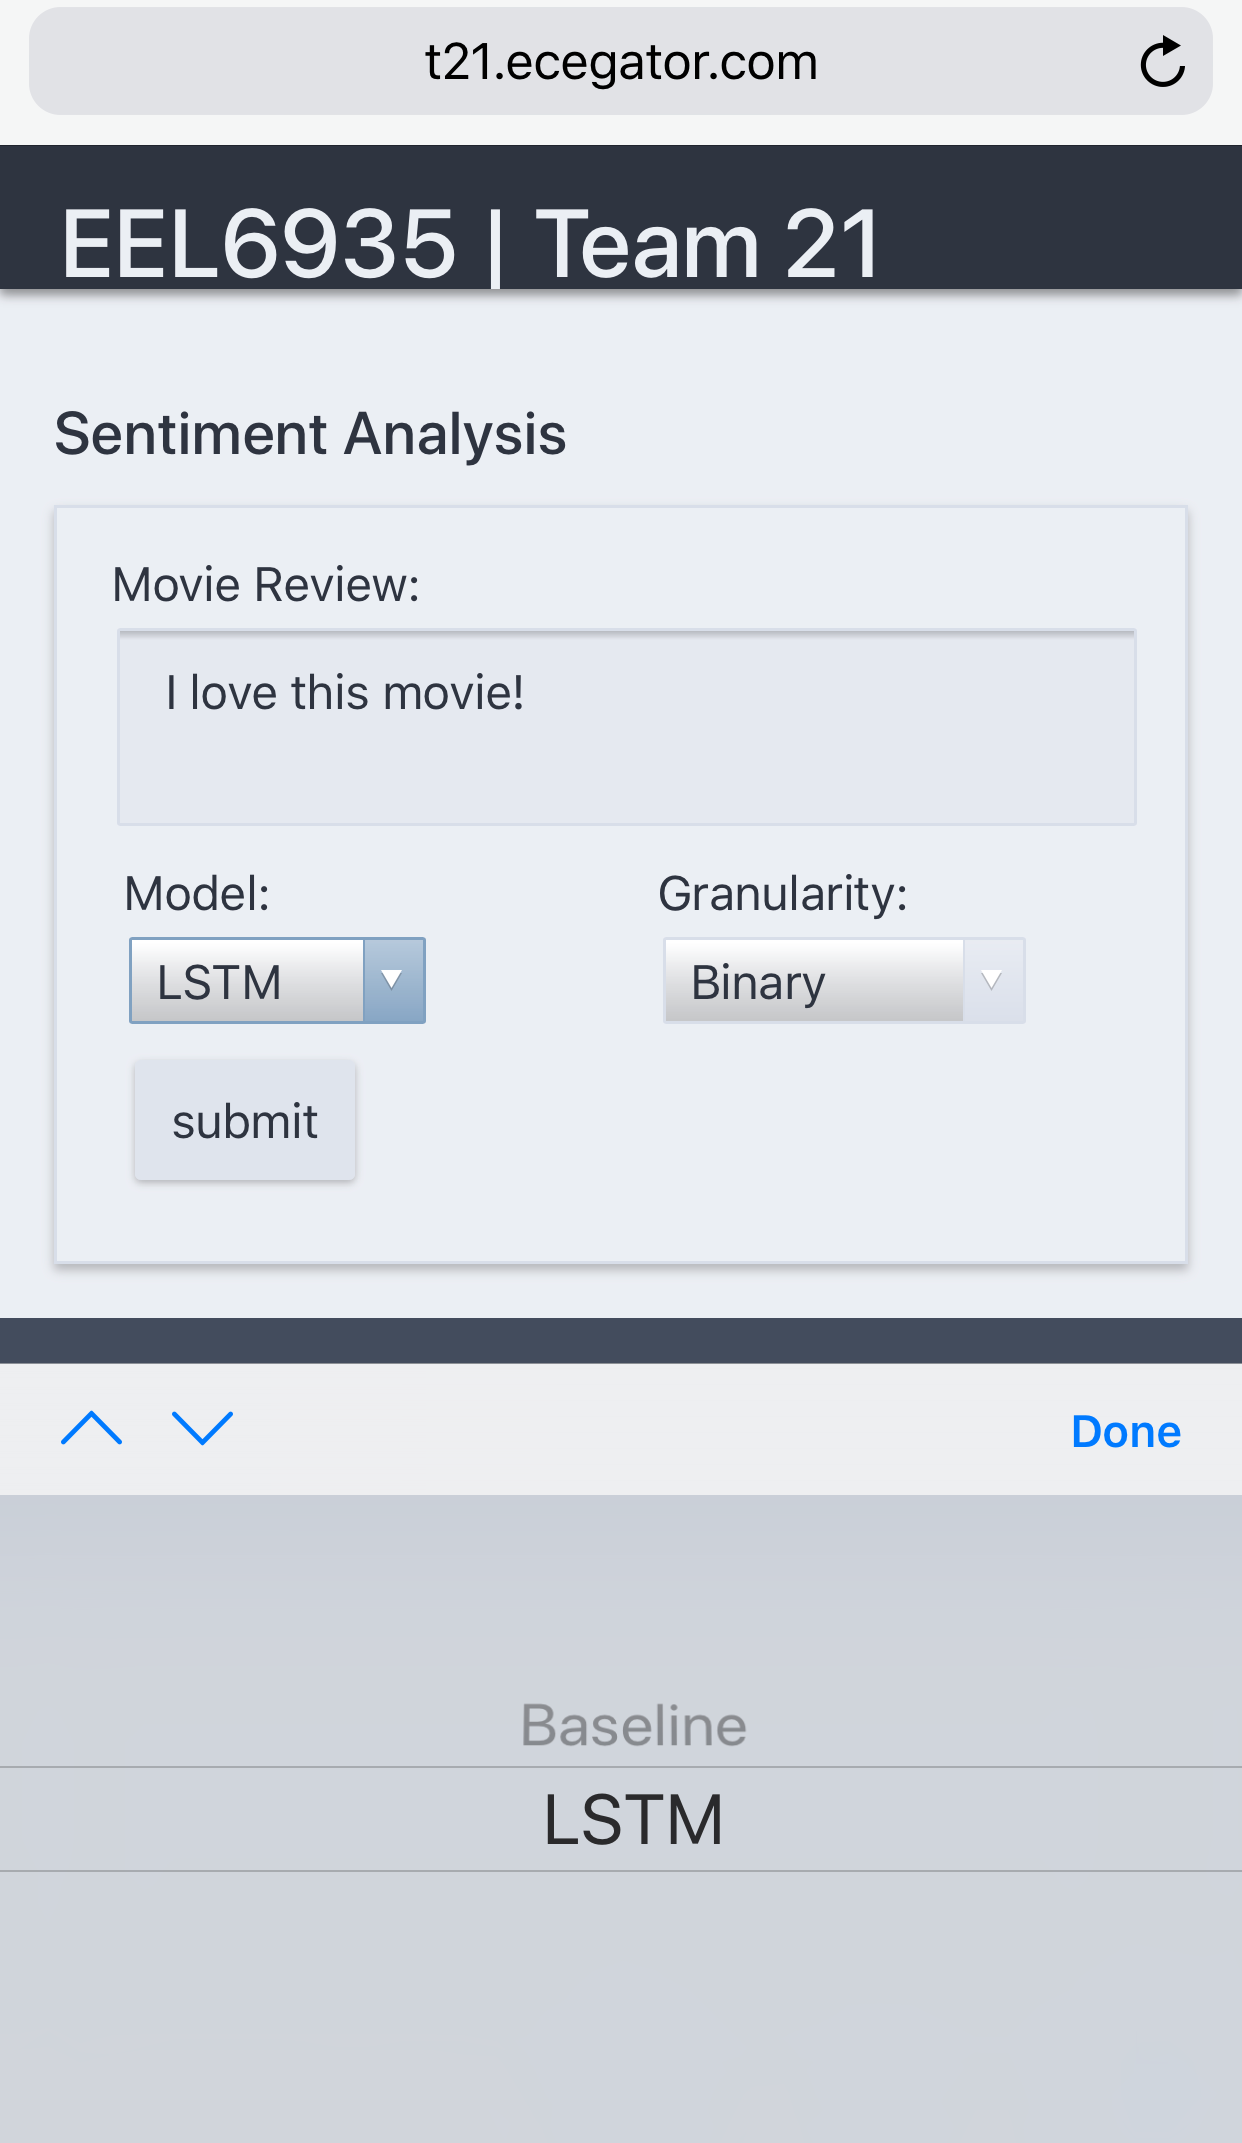
\includegraphics[width=0.9\textwidth]{figure/flask_input}
    \end{column}
    \begin{column}{0.3\textwidth}
        \center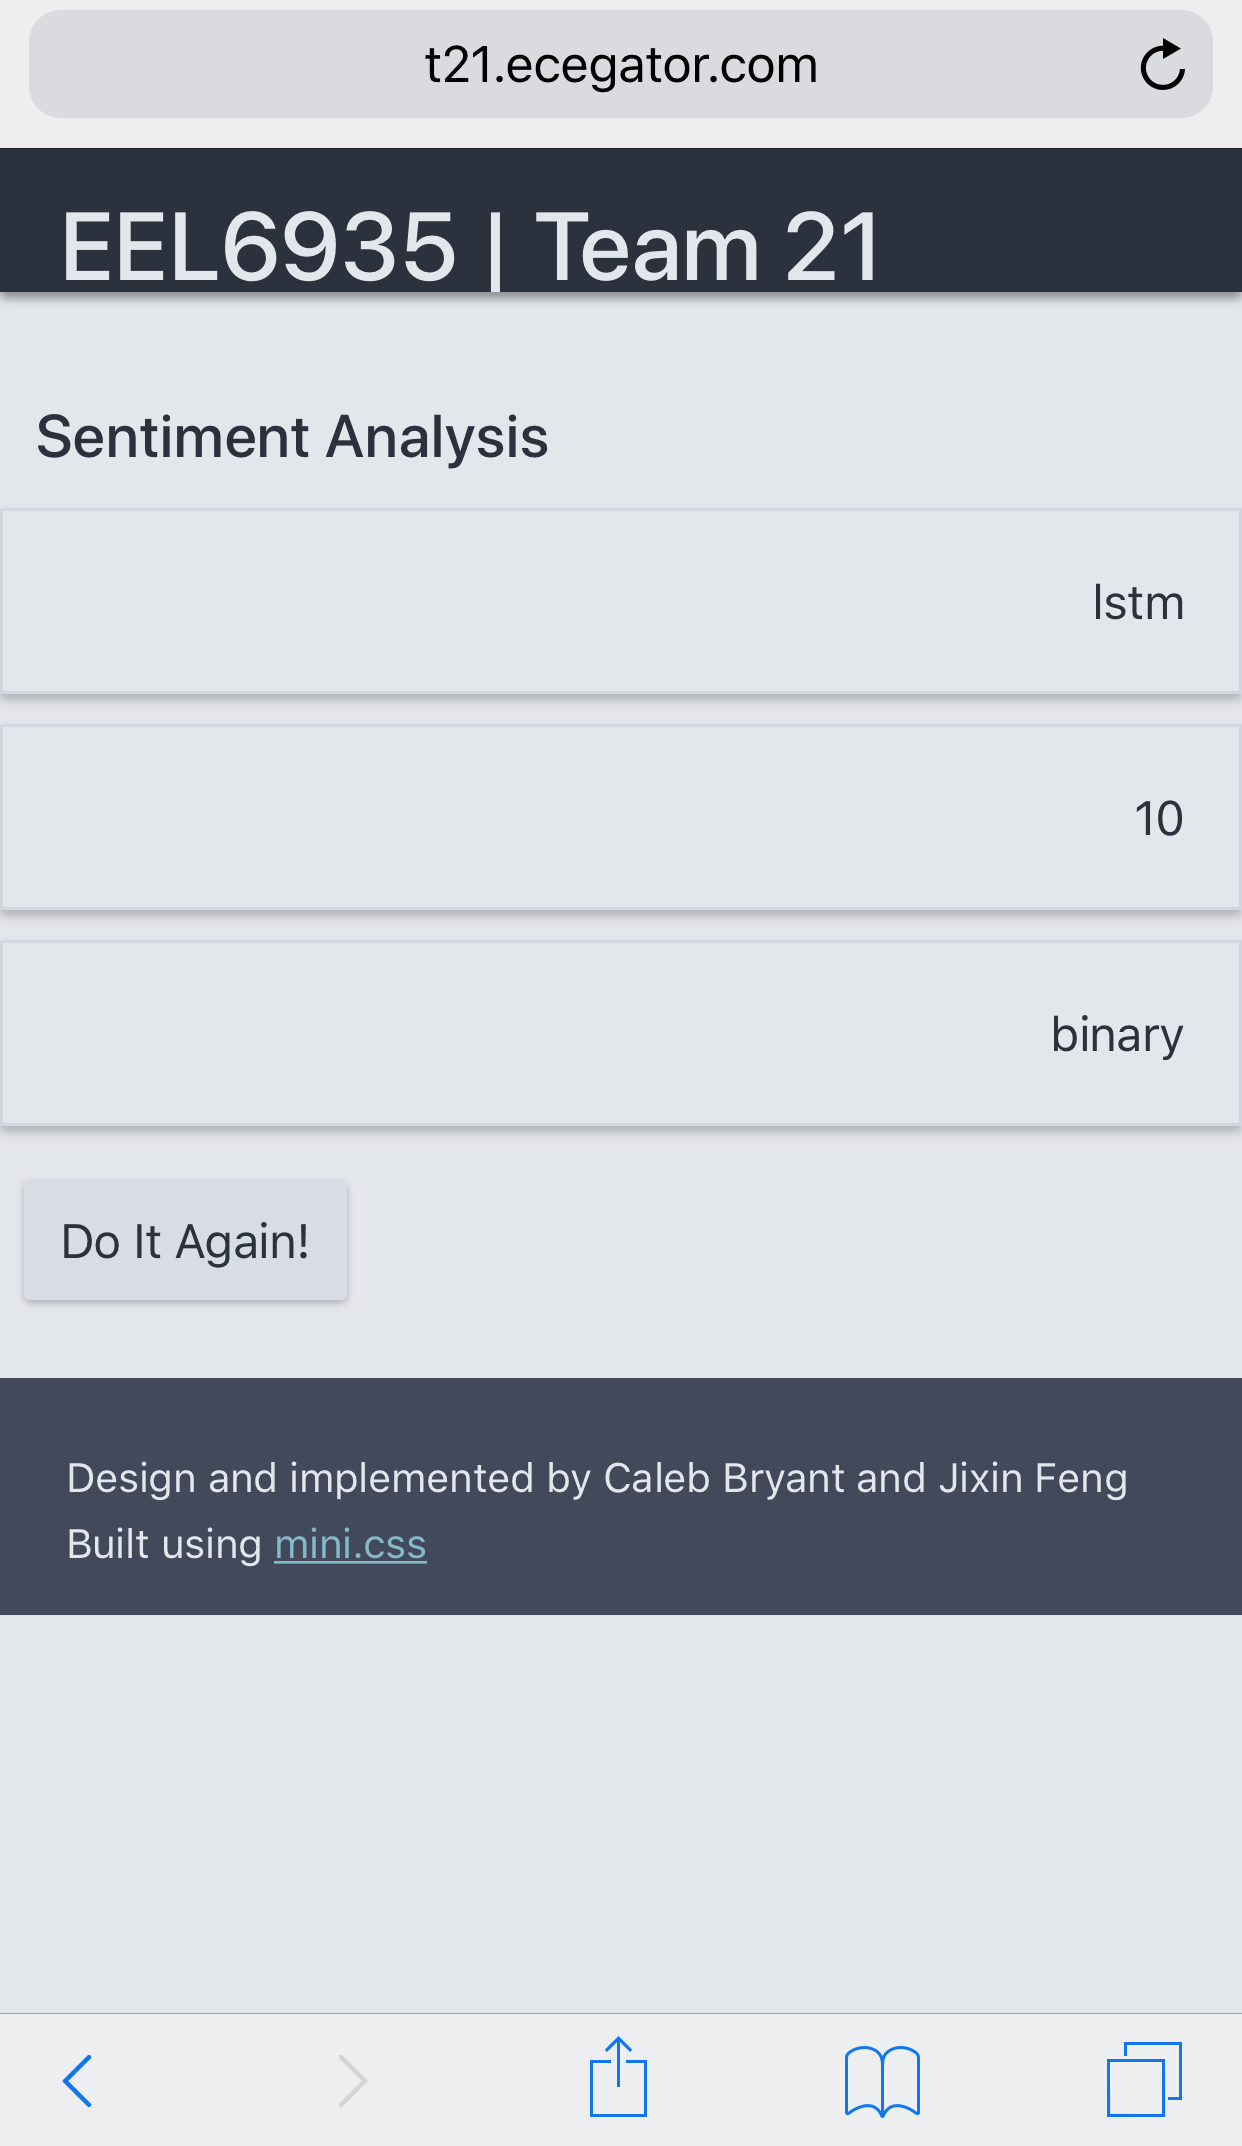
\includegraphics[width=0.9\textwidth]{figure/flask_output}
    \end{column}
    \end{columns}
\end{frame}

\begin{frame}
\frametitle{More About Us}
\begin{center}
\begin{tabular}{ccc}

\includegraphics[width=0.3\linewidth]{figure/qr_github} &  
\includegraphics[width=0.3\linewidth]{figure/qr_website} & 

\includegraphics[width=0.3\linewidth]{figure/qr_youtube} \\
\texttt{Code Repo} & \texttt{Web App} & \texttt{Video Demo}
\end{tabular}
\end{center}
\end{frame}

\begin{frame}

\includegraphics[width=\textwidth]{figure/dt180331}
\Huge{Thank You!}\\
\small{Questions?}\\
\end{frame}
\end{document}
